The call to \lst{nrn_fixed_step_thread()} implements a single time step for the set of cells on a thread, and accounts for over 99\% of all wall time. When discussing \emph{the algorithm} here, the focus is on the algorithm as implemented: with a higher level mathematical description of the algorithm proper where required to help understanding.

%%%%%%%%%%%%%%%%%%%%%%%%%%%%%%%%%%%%%%%%%%%%%%%%%%%%%%%%%%%%%%%%%%
\subsubsection{Spatial Discretization and Cable Equation}
%%%%%%%%%%%%%%%%%%%%%%%%%%%%%%%%%%%%%%%%%%%%%%%%%%%%%%%%%%%%%%%%%%
We first look at the spatial discretization of the partial differential equation (PDE) in \neuron. We consider a partial differential equation in one dimension with the general form
\begin{equation}
     C\pder{V}{t} + I = f \pder{}{x} \left( g\pder{V}{x} \right)
\end{equation}
where $f$ and $g$ are functions of the spatial dimension $x$ (they are functions of \emph{cable radius} in this model). The value of $I$ is dependent on the voltage $V$.

The spatial and temporal discretization used in Neuron is finite difference with a Crank Nicholson time stepping scheme. The time stepping scheme has an odd form, that differs slightly from the scheme presented here. However, the exposition here adequately characterizes the code.

\emph{Finite Difference Methods in Heat Transfer, Second Edition} By Necati Ozisik (1994) gives the following finite difference discretization
\begin{align}
    \dx \left(\at{C} \frac{\attplus{\at{V}} - \att{\at{V}}}{\dt} + \attplushalf{\at{I}} \right)
    &=\nonumber \\
    & \at{f} \theta
            \left[
                \atminushalf{g} \frac{\atminus{V}^{n+1}-\at{V}^{n+1}}{\dx}
              + \atplushalf{g}  \frac{\atplus{V}^{n+1}-\at{V}^{n+1}}{\dx}
            \right] \nonumber \\
            + & \at{f} (1-\theta)
            \left[
                \atminushalf{g} \frac{\atminus{V}^{n}-\at{V}^{n}}{\dx}
              + \atplushalf{g}  \frac{\atplus{V}^{n}-\at{V}^{n}}{\dx}
            \right]
        \label{eq:cableDiscretization}
\end{align}

where the parameter $\theta$ can be used to determine the time stepping scheme ($\theta=0$ explicit, $\theta=1$ implicit, $\theta=1/2$ Crank-Nicholson).

Note that the quantity $I$ depends on the value of $V$. These values have to be evaluated to form coefficients in the linear system that is to solved at each time step. The approach taken by Neuron is the evaluate them at a half time step value at $t+\dt/2$, denoted $\attplushalf{\at{I}}$, by implicitly solving for a half step, then performing an explicit half step.

With a Crank Nicholson time stepping scheme, i.e. $\theta=1/2$, the terms on the right hand side of \eq{eq:cableDiscretization} simplify to
\begin{align}
        \frac{\at{f}}{2}
        &\left\{
            \left[
                \atminushalf{g} \frac{\atminus{V}^{n+1}-\at{V}^{n+1}}{\dx}
              + \atplushalf{g}  \frac{\atplus{V}^{n+1}-\at{V}^{n+1}}{\dx}
            \right]
        \right. \nonumber \\
        +
        &\left.
            \left[
                \atminushalf{g} \frac{\atminus{V}^{n}-\at{V}^{n}}{\dx}
              + \atplushalf{g}  \frac{\atplus{V}^{n}-\at{V}^{n}}{\dx}
            \right]
        \right\} \label{eq:crankNichRHS}
\end{align}

Substituting the spatial discretization in~\eq{eq:crankNichRHS} into~\eq{eq:cableDiscretization} and rearranging gives a tri-diagonal linear system with the form
\begin{equation}
    \at{a} \atplus{V}^{n+1} + \at{d} \at{V}^{n+1} + \at{b} \atminus{V}^{n+1} = \at{r}
\end{equation}
where the diagonals in the matrix are defined
\begin{align}
    \at{a}  &=  -\frac{\at{f}\atplushalf{g}}{2\dx^2} \\
    \at{b}  &=  -\frac{\at{f}\atminushalf{g}}{2\dx^2} \\
    \at{d}  &=  \frac{\at{C}}{\dt} + \frac{f}{2\dx^2}\left[\atminushalf{g}+\atplushalf{g}\right] \nonumber\\
            &=  \frac{\at{C}}{\dt} - ( \at{a} + \at{b} ) \\
\intertext{and}
    \at{r}  &=  \frac{\at{C}}{\dt} \at{V}^n - \at{I} + \frac{\at{f}}{2\dx^2}
                    \left[
                        \atminushalf{g} \left( \atminus{V}^{n} - \at{V}^{n} \right)
                        +
                        \atplushalf{g}  \left( \atplus{V}^{n}  - \at{V}^{n} \right)
                    \right] \nonumber\\
            &=  \frac{\at{C}}{\dt} \at{V}^n
                - \at{I}
                - \at{a} \left( \atminus{V}^{n} - \at{V}^{n} \right)
                - \at{b} \left( \atplus{V}^{n}  - \at{V}^{n} \right)
\end{align}

It is important to note that the coefficients in the linear system are constant in time. In practice the off-diagonal entries in $\vv{a}$ and $\vv{b}$ are computed once at start up. The values on the diagonal, i.e. those in $\vv{d}$ are overwritten when solving the linear system using Thomas' algorithm. They are reconstructed using the values stored in $\vv{a}$ and $\vv{b}$
%%%%%%%%%%%%%%%%%%%%%%%%%%%%%%%%%%%%%%%%%%%%%%%%%%%%%%%%%%%%%%
\subsubsection{Not quite one-dimensional: trees \& branching}
%%%%%%%%%%%%%%%%%%%%%%%%%%%%%%%%%%%%%%%%%%%%%%%%%%%%%%%%%%%%%%
In the previous subsection a one-dimensional model and it's discretization were described. We will now extend this description to handle branching, whereby the domain is composed of a series of one-dimensional \emph{sections}, that are joined at branch points to form a tree. \hilight{Note: I don't discuss how the equations are modified to handle the nodes at branches, because that doesn't impact the discussion on the implementation.}

A small tree structure is illustrated in \fig{fig:tree}(a). It is important to note that the graph formed by the branching sections is a true tree, i.e. it has no circuits (once a section has branched, the branches can not ``rejoin'').

\begin{figure}[htp!]
\centering
\includegraphics[width=0.6\textwidth]{./images/tree.pdf}
\\{\normalsize (a)}\\
\includegraphics[width=\textwidth]{./images/discrete_a.pdf}
\includegraphics[width=\textwidth]{./images/discrete_b.pdf}
\includegraphics[width=\textwidth]{./images/discrete_c.pdf}
\includegraphics[width=\textwidth]{./images/discrete_d.pdf}
\includegraphics[width=\textwidth]{./images/discrete.pdf}
\\{\normalsize (b)}
\caption{Numbering of nodes and edges for Hines algorithm. (a) The high level branch and connection numbering scheme, with the branch nodes and sections numbered; (b) the numbering of individual nodes in the fully discretized domain with 5 segments per section.}
\label{fig:tree}
\end{figure}

Some terms used in discussing the tree structure in \fig{fig:tree} are:
\begin{itemize}
        \item \textbf{section} a branch in the tree structure, which corresponds to the one-dimensional line segmant between branch points. These are numbered $s*$ in \fig{fig:tree}(a).
        \item \textbf{branch} same definition as section.
        \item \textbf{node} a point in the spatial discretization. These are numbered in \fig{fig:tree}(b).
        \item \textbf{branch node} a node where two branches join. These are the blue points denoted $n*$ \fig{fig:tree}(a).
        \item \textbf{terminal branch} a branch that is one node that has one end that is connected to no other branches.
        \item \textbf{terminal node} a node that lies at the end of a branch that connects to no other branches. These correspond to $n1$, $n4$, $n5$ and $n6$ in \fig{fig:tree}(a).
\end{itemize}

The first step of the spatial discretixation is to discretize each one-dimensional section. Then the nodes are numbered using a scheme that gives the matrix a sparsity structure that allows the linear system to be solved in linear time, equivalent to Thomas algorithm.

The numbering scheme is as follows
\begin{enumerate}
\item
    A \emph{terminal branch} of the tree is selected, and its nodes are numbered with the terminal node last.
    The node numbered 1 is referred to as the \emph{root node} of the tree, and is shown in red in \fig{fig:tree}(b).
\item
    The tree is then traversed, with the nodes on each individual edge numbered such that the node index is higher for nodes further from the root. The sequence of steps illustrated in \fig{fig:tree}(b) shows the numbering applied in this manner as each branch of the tree is visited.
\end{enumerate}
A data-structure and algorithm for building the tree in \fig{fig:tree} are shown in \ap{appendix:treesource}. The source code for this was used to generate the images in this document.

The tree and it's corresponding matrix representation have the following properties:
\begin{itemize}
\item
    Every node has exactly one parent, except for the root node. In all cases the index of the parent $p_i$ of node $i$ is less than the index of the node, i.e. $p_i<i,~\forall\,i\in\left\{1,2,\dots,N\right\}$, where $N$ is the total number of nodes.
\item
    Non-terminal nodes have at least one child, i.e. nodes that have it as a parent, with branch nodes having one child for each branch in their subtree.
\item
    It is only necessary to store the parent indexes, the $p_i$ values, for each node in the tree.
\item
    The sparsity pattern of the linear system associated with this numbering has the following properties:
    \begin{itemize}
    \item
        The sparsity pattern is symmetric.
    \item
        the diagonal values are all nonzero.
    \item
        their is exactly one off diagonal value in each row of the lower triangle at $a_{ik}$, where $k=p_i$.
    \item
        their is exactly one off diagonal value in each column of the upper triangle at $a_{ki}$, where $k=p_i$.
    \end{itemize}
\item
    The sparsity pattern for the network in \fig{fig:tree}(b) is shown in \fig{fig:sparsity}. The pattern matrix was generated from the code in \ap{appendix:treesource}.
\item
    A matrix with this sparsity pattern can be stored with three vectores, $\vv{a}$, $\vv{b}$ and $\vv{c}$, where:
    \begin{align}
        a_i &= A_{ki} \\
        b_i &= A_{ik} \\
        d_i &= A_{ii}
    \end{align}
    where $k=p_i$.
\end{itemize}

\begin{figure}[htp!]
\centering
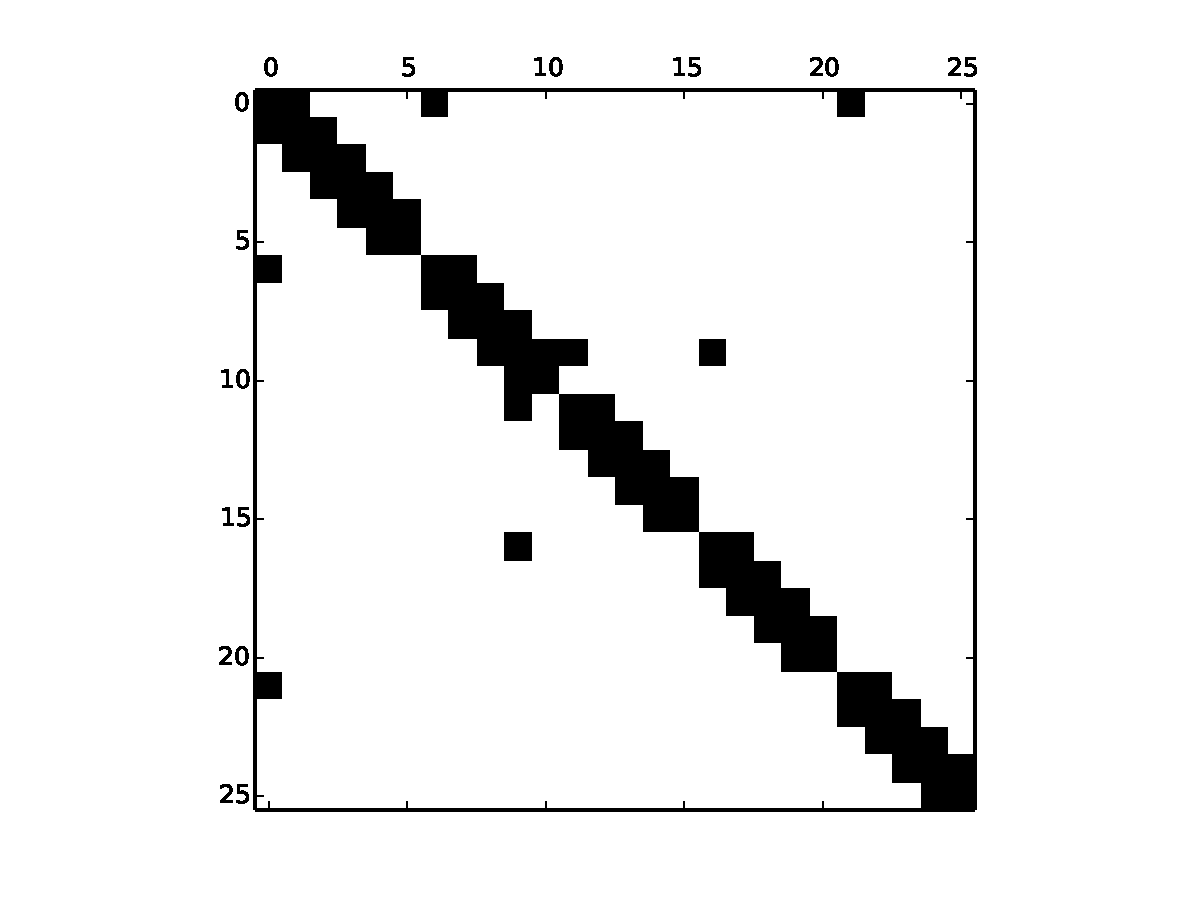
\includegraphics[width=0.5\textwidth]{./images/sparsity.pdf}
\caption{Sparsity pattern of the matrix corresponding to the tree numbering in \fig{fig:tree}.}
\label{fig:sparsity}
\end{figure}


These linear systems can be solved very efficiently, in linear $O(N)$ time, using an algorithm that is equivalent to the Thomas algorithm for solving tri-diagonal systems. This algorithm, called Hines algorithm, proceeds by eliminating the nonzero entries in the upper triangle of $A$. Recall the matrix property that there is only one non-zero value in each column of the upper triangle at $A_{ki}$, which is stored in $a_i$.
\begin{equation}
\left(
        \begin{array}{ccc}
            A_{kk} & \dots      & A_{ki} \\
        \vdots     & \ddots     & \mathbf{0} \\
            A_{ik} & \mathbf{0} & A_{ii}
        \end{array}
\right)
\text{which is stored as:}
\left(
        \begin{array}{ccc}
            d_k & \dots      & a_i \\
        \vdots  & \ddots     & \mathbf{0} \\
            b_i & \mathbf{0} & d_i
        \end{array}
\right)
\end{equation}
The value $a_i$ and can be zeroed out with a row operation
\begin{equation*}
    \text{row}_k \leftarrow \text{row}_k - a_i/d_i\cdot\text{row}_i.
\end{equation*}
In practice the value of $a_i$ is not changed, and only the diagonal entry has to be modified
\begin{equation*}
d_k \leftarrow d_k - a_i/d_i\cdot b_i.
\end{equation*}
The forward substitution is then used to determine the solution. The forward and backward substitution are implemented in Julia in \ap{appendix:hinessource}.


